\input{common}
\title{Введение в GNU/Linux\\Командная строка}

\begin{document}
\begin{frame}
 \frametitle{}
 \titlepage
\end{frame}

\section{Интерфейс командной строки}
\mode<all>{% Тема. Командная строка. 
% Показать примеры использования. Рассказать о преимуществах и недостатках в
% сравненни с графическим "оконным" интерфейсом. 
% Ознакомить с назначениме  эмулятора терминала и об реализациях.

\begin{frame}{Примеры использования командной строки}
	\begin{columns}
	\column{0.5\textwidth}
        \begin{itemize}
            \item чаты
            \item компьютерные игры Quake, DotA
            \item операционные системы
        \end{itemize}
	\column{0.5\textwidth}
	% insert picture of Quake 
    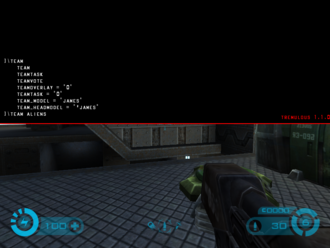
\includegraphics[height=0.4\textheight]{../../slides/cmdline/330px-Tremulous_console.png}
	\end{columns}
\end{frame}

\begin{frame}{Преимущества командной строки}
	\begin{itemize}
		\item Работа через сеть либо RS232
		\item Быстрый доступ к командам системы
		\item Легче отладка сообществом
		\item Легкость автоматизации
	\end{itemize}
\end{frame}

\begin{frame}{Недостатки командной строки}
	\begin{itemize}
		\item Oтсутствуют возможности обнаружения (discoverabililty)
		\item Необходимость изучения синтаксиса команд и запоминания сокращений.  (синтаксис может различаться)
		\item Без автодополнения, ввод длинных и содержащих спецсимволы параметров с клавиатуры может быть затруднительным
		\item Отсутствие «аналогового» ввода.
	\end{itemize}
\end{frame}

\begin{frame}{Эмуляторы терминала в графическом режиме}
	\begin{itemize}
		\item xterm
		\item rxvt
        \item gnome-terminal
        \item konsole
        \item Yakuake (Yet Another Kuake)
	\end{itemize}
\end{frame}
\note { 
Примеры приложений которые лучше выглядят в графическом режиме браузер,
редакторы видео и графики. Поэтому пользователь при работе, как правило,
совмещает оба интерфейса: использует графическое окружениe в сочетании с
интерфейсом командной строки. 
В графическом окружении интерфейса командной строки предоставляют приложения -
эмуляторы терминала. 
реализации - для графической системы X Window xterm, rxvt. Для GNOME
gnome-terminal, для KDE konsole, Yakuake (Yet Another Kuake выезжает по нажатии
тильды ~ как Quake)  
Дополнительные замечания:
Терминал - устройство для ввода вывода информации, уже устарел.
Графические приложения можно запускать из командной строки. 
}
}

\section{ Командная оболочка(shell) }
\begin{frame}
\frametitle{}
 \begin{center}
   {\Large Командная оболочка(shell) }
 \end{center}
\end{frame}


\mode<all>{\begin{frame}[fragile]{Оболочка операционной системы}

     \begin{block}{Оболочка операционной системы}
     (от англ. shell «оболочка») \alert{интерпретатор команд} операционной системы, обеспечивающий интерфейс для взаимодействия пользователя с функциями системы.  
     \end{block}
     Что такое Unix shell?
     \begin{itemize}
        \item Обычная программа, запускающаяся после входа в систему
        \item Интерактивный командный интерпретатор
        \item Платформа интеграции (для утилит)
        \item Язык программирования
     \end{itemize}

	\pause
	\vspace{0.5in}
	Пример shell из  Windows-world --  cmd.exe, PowerShell
	\vspace{0.5in}
	Минимальный дистрибутив Linux -- ядро + shell 

\end{frame}
\note{   
     Как вы помните задачи ядра - управление процессами и потоками, управление
     памятью, Управление файлами, Разграничение доступа, мониторинг и
     конфигурация. Shell обеспечивает пользователю  интерфейс доступа к этим функциям ядра.    
     Как Интерактивный командный интерпретатор shell предосталяет средства:
     редактора командной строки, часто со средствами упрощающими ввод команд
     такими как  горячие клавишами, автодополнение, история команд и поиск по
     истории, сокращения команд (aliases), сокращения путей к файлам c помощью
     спецсимволов. 
     Как Платформа интеграции предоставляет средства пренаправления
     ввода/вывода, каналы (pipes), и возможность создавать скрипты.
     Одновременно является языком программирования, но эту часть будем
     рассматривать позже. 
}

\begin{frame}[fragile]{Основные типы shell в Unix}
  \begin{itemize}
    \item Bourne shell совместимые (POSIX-совместимые)
      \begin{itemize}
        \item \textbf{sh} исходная bourne shell (Steve Bourne, 1978)
        \item \textbf{ksh} Korn shell (David Korn, 1983)
        \item \textbf{ash} $[$BSD$]$ Almquist shell (Kenneth Almquist,1989)  
        \item \textbf{bash} $[$GPL$]$ Bourne-again shell (Brian Fox, 1989)
        \item \textbf{zsh} $[$BSD$]$ Z shell (Paul Falstad,1990)
        \item \textbf{/bin/sh} Указывает на POSIX-совместимую shell
      \end{itemize}
  \item C shell совместимые
      \begin{itemize}
        \item \textbf{csh}  Исходная С shell (Bill Joy, 1978)
        \item \textbf{tcsh} $[$BSD$]$ TENEX C shell (Ken Greer, 1981)
       \end{itemize}
  \end{itemize}
\end{frame}

\note { 
Существуют  Рассмотрим наиболее распрастраненные реализации оболочек: 
Разделяются на две группы POSIX-совместимые и несовместимые. 
sh — оригинальный шелл Борна;
bash (bourne again shell) (эмуляция совместимости POSIX[1]) расширенная Борном свободная (разработанная в рамках проекта GNU). Стандартная оболочка в Linux.

C shell — (несовместима с POSIX shell) оболочка, с синтаксисом на основе Си,
созданная Университетом Беркли в рамках проекта по реализации BSD Unix.
    csh (C-Shell) — оболочка из состава дистрибутива BSD, имеет Си-образный синтаксис и не является POSIX-совместимой. Впервые введены возможности управления заданиями и произведены другие улучшения.
    tcsh (csh) — реализация csh с интерактивными возможностями, не уступающими bash[1]. Удобна для интерактивной работы. Совместима с csh.
}

\begin{frame}[fragile]{Какие могут быть различия между shell}
  \begin{itemize}
    \item Интерактивные возможности
    \item Платформы
    \item Поиск соответствий строк и имён файлов
    \item Программные возможности
    \item Cовместимость оболочек между собой
\end{itemize}
\end{frame}
/note {
Интерактивные возможности - клавиатурные сокращения, средства автодополнения, настройки по умолчанию
Платформы - на чем работают оболочки. bash - кросплотформенная, zsh - нет. 
Программные возможности - различный синтаксис, bashизмы, функции определяются
по разному, средства программирования циклы, списки, массивы. Отсюда
совместимость между собой. 
Мы будет придерживаться синтаксиса оболочки bash, т.к. она по умолчанию
используется в дистрибутивах Linux.  Это позволит создать базу, с
котороый вы легко сможете перейти на подходящие вам варианты. 
}


\begin{frame}[fragile]{Как работать с командной строкой}
  \begin{itemize}
    \item 
	Находим приглашение командной строки
	\$, \#, user@host:~\$
    \item
	Вводим имя команды, опции, аргументы, запускаем на выполнение нажатием <Enter>
   \end{itemize}

	Что такое команды?
  \begin{itemize}
    \item исполняемая программа (бинарный файл, скрипт)
    \item встроенные в оболочку команды (shell built-ins)
    \item функция оболочки
    \item сокращение команды (an alias) 
  \end{itemize}
\end{frame}
\note {
Система ожидает ввода команды, показывая приглашение командной строки.
Пользователь вводит команды опции аргументы и нажимает <Enter>. 
Опции - модификаторы поведения программы.  
Аргументы - то над чем производятся действия.
}


\begin{frame}[fragile]{Маленькое упражнение}
Определить список установленных оболочек в системе.
\begin{lstlisting}[language=bash]
cat /etc/shells
ls -l <filename> # для каждого элемента /etc/shells
readlink -e <filename> 
\end{lstlisting}
Командой type определить какой тип команды (встроенная в оболочку или внешняя программа)
\begin{lstlisting}[language=bash]
type type
type dmesg
type ls
type -a test
\end{lstlisting}
\end{frame}


}
\begin{frame}
\frametitle{}
 \begin{center}
   {\Large Help }
 \end{center}
\end{frame}
\mode<all>{\begin{frame}[fragile]{Получение помощи}
  \begin{itemize}
    \pause
    \item \textbf{man} - помощь по внешним командам
    \pause
    \item \textbf{help} - помощь по внутренним командам bash (также man bash)
    \pause
    \item \textbf{info} - расширенная помощь по некоторым командам (texinfo format)
      \begin{itemize}
       \item   Попробовать {\tt info coreutils}
       \item   Справка по навигации -- нажать h
      \end{itemize}
  \end{itemize}
\end{frame}

\begin{frame}[fragile]{Основное о man}
\begin{columns}
	\column{2.2in}
		\begin{itemize}
			\item Прочитайте {\tt man man} !
			\item Apropos {\tt man -k <слово>}
			\item Разделы (sections)
				\begin{itemize}
					\item[1] Основная секция(юзерские программы)
					\item[2] Syscalls
					\item[3] С library
					\item[5] Конфигурационные файлы
					\item[8] Системные службы
				\end{itemize}
		\end{itemize}
	  \textbf{Замечание}

	  Обычно внутри страницы работает поиск с помощью '/'
	\pause 
	
	\column{1in}
		\begin{block}{Попробовать}
			\begin{lstlisting}
man -k printf
man 3 printf
man 1 printf
man -a printf
			\end{lstlisting}
		\end{block}
	\end{columns}
\end{frame}


}
\begin{frame}
\frametitle{}
 \begin{center}
   {\Large Навигация по файловой системе }
 \end{center}
\end{frame}
\mode<all>{\begin{frame}{Навигация по файловой системе}
      \begin{itemize}
		  \item {\tt ls} -- список файлов в (текущей по умолчанию) директории (man ls)
		  \item {\tt cd} -- смена текущей директории (help cd)
		  \item {\tt pwd} -- имя текущей директории (help pwd)
      \end{itemize}
\end{frame}

\begin{frame}[fragile]{Команды для работы с файлами}
	\begin{itemize}
		\begin{columns}
		\column{0.2\textwidth}
			\item touch
			\item ln
			\item mkdir
			\item mknod
			\item mkfifo

		\column{0.2\textwidth}
			\item cp
			\item mv
			\item install
			\item rm
			\item rmdir
			\item file

		\column{0.4\textwidth}
			\begin{block}{Упражнение}
				\begin{enumerate}
					\item Создать иерархию директорий
						\begin{lstlisting}
dir1/dir1.1/dir1.1.1
dir1/dir1.2/dir1.2.1
dir1/dir1.2/dir1.2.2
						\end{lstlisting}
					\item Внутри каждой создать файл
					\item Удалить все созданное
				\end{enumerate}
			\end{block}
			
		\end{columns}
	\end{itemize}
\end{frame}


}

\mode<all>{\begin{frame}{Файловая структура}
	
	{\center "Дерево внутри дома?" (c) Шрек}
		
	\begin{columns}
	\column{0.2\textwidth}
		\includegraphics[height=0.8\textheight]{../../slides/fs/01-lhs.png}
		
	\column{0.7\textwidth}
		\begin{itemize}
			\item Директории
			\item Обычные файлы
			\item Симлинки
			\item Хардлинки
			\item Файлы устройств
			\item FIFO
			\item сокеты
		\end{itemize}
	\end{columns}
\end{frame}
}

\mode<all>{\input{../../slides/cmdline/bash-intro}}


\begin{frame}{Задание на дом}
\begin{block}{}
vimtutor ru
\end{block}
\end{frame}

\end{document}

